\documentclass[12pt,a4paper]{article}
\usepackage[utf8]{inputenc}
\usepackage{graphicx}
\usepackage{color}
\usepackage[magyar]{babel}
\usepackage{listings}
\usepackage{float}

\usepackage{enumerate}
\usepackage{tikz}
\usetikzlibrary{shapes,arrows}
\usetikzlibrary{positioning}
\usetikzlibrary{arrows.meta}

\tikzset{
block/.style = {draw, fill=white, rectangle, minimum height=3em, minimum width=3em},
tmp/.style  = {coordinate}, 
input/.style = {coordinate},
output/.style= {coordinate},
pinstyle/.style = {pin edge={to-,thin,black}
}
}
\usepackage[siunitx]{circuitikz} 
\renewcommand{\lstlistingname}{Lista}
\usepackage{hyperref}
\hypersetup{
	pdftitle={HA5KFU tanfolyam - Modulációs gyakorlat},
	pdfauthor={HA5KFU Rádióamatőr Klub},
	pdfsubject={HA5KFU tanfolyam},
	pdfcreator={latex},
	pdfkeywords={ },
	pdfpagemode=UseOutlines,
	pdfdisplaydoctitle=true,
	pdflang=hu,
	unicode
}
\usepackage{color} %red, green, blue, yellow, cyan, magenta, black, white
\definecolor{mygreen}{RGB}{28,172,0} % color values Red, Green, Blue
\definecolor{mylilas}{RGB}{170,55,241}
\lstset{language=Matlab,%
	basicstyle=\scriptsize\ttfamily,
    %basicstyle=\color{red},
    breaklines=true,%
    morekeywords={matlab2tikz},
    keywordstyle=\color{blue},%
    morekeywords=[2]{1}, keywordstyle=[2]{\color{black}},
    identifierstyle=\color{black},%
    stringstyle=\color{mylilas},
    commentstyle=\color{mygreen},%
    showstringspaces=false,%without this there will be a symbol in the places where there is a space
    numbers=left,%
    numberstyle={\tiny \color{black}},% size of the numbers
    numbersep=9pt, % this defines how far the numbers are from the text
    emph=[1]{for,end,break},emphstyle=[1]\color{red}, %some words to emphasise
    %emph=[2]{word1,word2}, emphstyle=[2]{style},    
}

\pagestyle{plain}
\sloppy
\begin{document}
\begin{center}

\includegraphics[width=300pt,keepaspectratio]{figures/ha5kfu.eps}
\\[0.5cm]
Rádióamatőr tanfolyamot segítő jegyzet, egyelőre kidolgozás alatt \\
Szabó Áron HA1FLX, Kiss Ádám HA8KDA, Bazsó Márton HA7BM % Feel free to add yourself
\\[1cm]

{\huge \bfseries Modulációs gyakorlat \\[2cm]}



\end{center}

\renewcommand{\contentsname}{Tartalom}\tableofcontents 
\newpage

\newpage

\section{Bevezető}
A workshop célja bemutatni a különböző modulációs eljárások idő- és frekvenciatartománybeli viselkedését, illetve matematikai leírásukat. 

\section{Előkészületek}
A workshop Octave-ban és Matlab-ban is elvégezhető, a használt parancsok mindkettőben működőképesek.

\paragraph{Octave telepítés:} 
\begin{itemize}
	\item \textbf{GNU Octave telepítése:} \\\url{https://wiki.octave.org/Category:Installation}
	\item \textbf{Signal package telepítése:} Octave-on belül: 	\\
	\texttt{pkg install -forge signal}\\
	Ha ez valamiért nem működne, akkor Ubuntun command line-ból is telepítheted: \texttt{sudo apt-get install octave-signal}
\end{itemize}


\section{Elméleti összefoglaló}
\subsection{Keverés szükségessége}
Tegyük fel, hogy van egy modulált jelünk valahol a rádiós spektrumban. (Pl. 540 kHz-en a Kossuth rádió vagy a 12 GHz-en egy prémium műhold csatorna kedvenc szolgáltatónknál) Ezt szeretnénk venni. A vett jel szempontjából zavaró információ az összes többi adás, illetve az egyéb frekvenciákon mérhető zaj, ezeket szükséges kiszűrni a tökéletes vételhez. A probléma, hogy gyakorlatilag kivitelezhetetlen nagyon keskeny szűrő magas frekvenciákon. Például egy 1 MHz sávszélességű jelet kiszűrni GHz-es tartományban már lehetetlen. Az úgynevezett relatív sávszélesség (sávszélesség osztva sávközéppel) egy ezred. Sok gyakorlattal és minőségi alkatrészekből építkezve körülbelül egy tizedes relatív sávszélességig tudunk megvalósítani áramkört.\par
A problémát egy csellel oldjuk meg. Nagyjából kiszűrjük a jelet a saját sávjában, esetleg még erősítjük is (itt a sorrend lehet fordított!). Majd egy keverőt helyezünk el. A keverő frekvenciában eltolja a bemeneti jelet az ő oszcillátor bemenetének frekvenciájával mindkét irányba. A nem használt keverési terméket kiszűrjük. (Kellően nagy keverési frekvencia esetén ez messze fog kerülni a használttól, így könnyű hozzá szűrőt tervezni). Így a jelünk alacsonyabb frekvenciára került, ahol már ugyan akkora ügyességgel és anyagminőséggel keskenyebb sávú szűrőt tudunk építeni. Ezzel a módszerrel ki tudjuk szűrni a számunkra fontos jel körül a többi zavaró jelet.
\subsubsection{Elgondolkodtató megjegyzések}
Létezik úgynevezett tükörfrekvencia. Ez az a sáv, amit a keverő ugyan arra a frekvenciára kever, mint a hasznos jelet -- ezt ki kell szűrni a keverés előtt, különben áthallás lesz két adó között. A keverő kimenetét középfrekvenciának szokták hívni, az ezt követő szűrőt KF szűrőnek. (Angolul intermediate freq, és IF filter). Ha hangolható a keverőnk oszcillátora, akkor a lefedett sáv nem lehet nagyobb a KF szűrő sávközepének kétszeresénél. Ha vevőt építünk, akkor érdemes először felfele keverni, azaz a magasabb frekvenciájú keverési terméket használni, ott szűrni, majd onnan lekeverni, mert így lesz a legnagyobb az ún. tükörszelektivitásunk. Digitális jeleknél is fennáll a fenti gondolatmenet, létezik úgynevezett digitális KF is.

\subsection{Keverés matematikája}
Vizsgáljuk csupán egy szinuszjelet, ennél összetettebb jel felfogható több szinusz összegeként, a lentiek igazak erre az esetre is, csak több példányban értelmezve
\par
Vegyünk egy vektort, ami forog körbe körbe. Vegyük ennek a vektor csücskének az egyik tengelyre vett árnyékát. A tengelyen a szinusz függvény szerint fog mozogni a pont. Ha ezt a tengelyen mozgó pontot egy ceruzára cseréljük, és a papírt elkezdjük a mozgására merőlegesen lehúzni egyenletes sebességgel, akkor egy ideális szinuszt fogunk kapni. Bizonyítást lásd Euler-tétel.
\par
A keverés során semmi mást nem teszünk, mint próbáljuk felvenni a sebességet a jellel. Azaz a vektor továbbra is forog úgy, ahogy forog, viszont a koordináta rendszert elkezdjük forgatni hozzá. Ha ugyan azon irányba, akkor különbségi keverést csinálunk, ha ellentétesbe, akkor összegzőt. (A valóságban persze a kettőt csak együtt tudjuk csinálni. Valós szinusszal keverünk, ami az Euler-tétel miatt két részre bontható, az egyik az egyik, a másik iránynak felel meg.) Ekkor elképzelhető, hogy a kapott szinuszunk lassul vagy gyorsul. Le tudjuk azonos sebesség esetén nullára is lassítani a látszólagos sebességét. Ekkor a szinusz és a koordináta-rendszerünk fázisától függően egy valamilyen álló fázisban látjuk a vektort.
\par
A koordináta-rendszert, amiben ábrázoljuk a lelassított szinusz, konstellációs diagramnak nevezzük. A vett jel (tfh. szinusz) vektorának a végpontját pedig konstellációs pontnak. Szokás a különböző konstellációs térnegyedekhez vagy ennél is finomabb felbontásokhoz digitális szimbólumokat is rendelni, amiket később (miután rászinkronizált a vevő az adó bitkibocsájtási ütemére) bitfolyamként tud értelmezni egy következő fokozat.

\subsection{Egyszerű modulációk konstellációs ábrája}
\paragraph{AM}
Amplitúdó modulált esetben a konstellációs pont szöge áll, azonban az amplitúdója változik. Amennyiben a szög folyamatosan nő enyhén, úgy frekvencia-hibánk van az adóhoz képest, az oszcillátorunk frekvenciája kicsit más.
\paragraph{PM}
Fázismodulációnál az adó néha fázist vált a jelében, ekkor nálunk a lekevert/visszalassított szinuszban is lesz egy fázisugrás. Amennyiben az elvárt szimbólumok helyei itt is egy kör mentén vándorolnak, úgy frekvenciahibánk van.
\paragraph{FM}
Frekvenciamodulációnál nem szoktuk lekövetni pontosan a frekvenciaváltozását a jelnek. Azt nézzük, hogy épp milyen ütemben gyorsul el tőlünk, vagy lassul vissza hozzánk. Felírva szögfüggvényekkel, hogy épp mekkora szögsebessége van az FM jelnek (ehhez kell az előző vektor értéke is) számolható egy érték, amit megfelelő konstanssal (hangerő) megszorozva már demoduláltuk is a jelet. A frekvenciahiba itt egy konstans eltolást jelent majd a demodulált jelben. Hang esetén ezt nem halljuk ki.

\subsection{IQ demodulátorok}
Az IQ demodulátornál egy szinusz és egy koszinusz jellel is megszorozzuk a bejövő jelünket. A szinusznak és a koszinusznak a frekvenciája megegyezik. Feltételezve, hogy a felső keverési termékeket külön-külön kiszűrjük, megkapjuk a visszalassítós keverést. Az I és Q jelet lehet külön-külön digitalizálni, ezen a ponton már nem is szükséges nagyon gyors analógból digitális átalakítás, hiszen lassú jelekkel dolgozunk. Az I és Q jelek mint koordináták fogják megmutatni, hogy épp merre mutat a vett jel vektora, plusz a való életben valamekkora zaj is fog megjelenni ezen túl. Az IQ jelek digitálisan feldolgozhatóak, elvégezhető a demoduláció. Ezen az elven alapszik a gyakran használt RTL-SDR működése is, amivel például a SMOG jeleit is lehet fogni.

\clearpage
\section{Feladatok}

\subsection{Szinusz jel generálása, ábrázolása}
Első feladatunk egy szinusz jel generálása lesz, melyet a \textit{sin()} függvénnyel tehetünk meg. Fontos, hogy ez a függvény egy adott érték szinuszát adja vissza, nekünk viszont egy időtartománybeli függvényre van szükségünk. 

Létre kell hoznunk tehát egy időtengelyt, aminek pontjaiban kiszámoljuk a függvény értékét. Ebből a szempontból fontos meghatározni a mintavételi frekvenciát ($F_s$), hiszen ebből az értékből számolható, hogy két minta közt mennyi idő fog eltelni. Válasszuk a mintavételi frekvenciát \textit{44 100 Hz}-re, ami a digitális audió jelfeldolgozásban használatos frekvencia, és a számítógép hangkártyáján könnyen lejátszható.

Ha a minta hosszát ($l$) másodpercben szeretnénk megadni, a minták számának ($N$) meghatározásához egyszerűen szorozzuk meg a másodperc értéket a mintavételi frekvenciával. A másodperc időtengelyt ($t$) úgy kaphatjuk meg, ha az \texttt{1:N} sorozatot elemenként elosztjuk a mintavételi frekvenciával (a transzponálásra azért van szükség, hogy oszlopvektort kapjunk). Ez után a szinusz jel egyszerűen kiszámolható: mivel a szinusz egy periódusa $2\pi$, a szinuszjel pillanatnyi értékét $t \cdot f \cdot 2\pi$-re kell választani, ahol $f$ a szinusz frekvenciája.

\begin{lstlisting}[frame=single,language=matlab,caption=Mintavételi frekvencia beállítása és szinuszjel előállítása]
Fs = 44100; % mintaveteli freki
l = 1.5; % minta hossza masodpercben
N = l * Fs, % mintak szama
f = 440; % 20 Hz-es lesz a jel
t = ( 1:N )' ./ Fs; % Ido oszlopvektora
y = sin( t * f * 2 * pi );
plot( t, y );
\end{lstlisting}

Ábrázoljuk a Plot függvénnyel időtartományban:

\begin{figure}[H]
\begin{center}
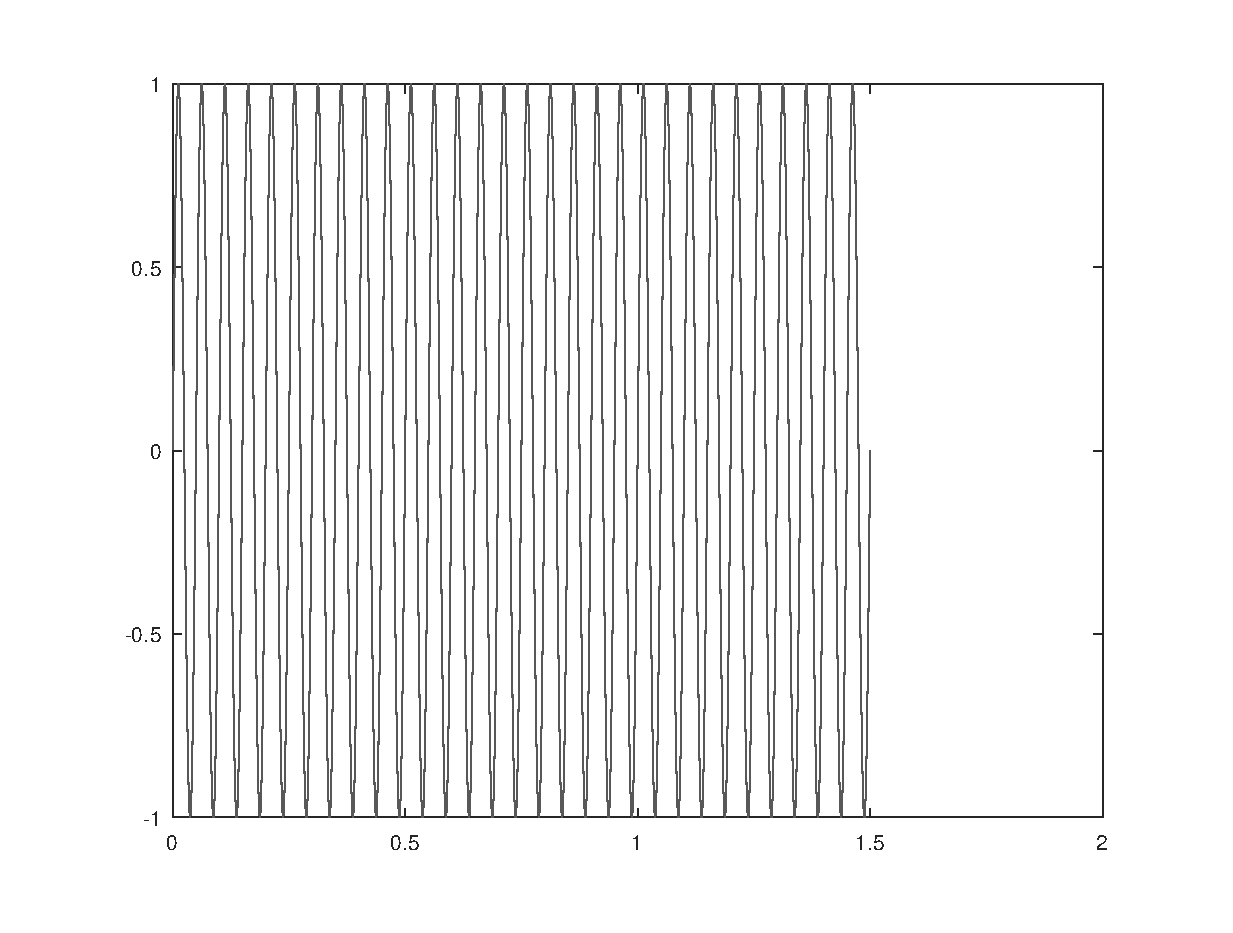
\includegraphics[width=8cm]{figures/modulaciok_workshop_szinusz.eps}
\caption{20 Hz-es szinusz függvény ábrázolása időtartományban}
\label{fig:szinusz}
\end{center}
\end{figure}

A 20 Hz-es jelet könnyen ábrázoltuk, de a hallható tartomány magasabb frekvencián van. Változtassuk a jel frekvenciáját 440 Hz-re (zenei A hang), és játsszuk ki a számítógép hangkártyáján a jelet:

\lstinline{soundsc(y, Fs); % Hang lejatszasa Fs mintaveteli frekvenciaval } 


Itt már több információt kapnánk a jelről, ha frekvenciatartományban, vízesés diagramon ábrázolnánk a jelet. A HA5KFU Octave gyakorlathoz csomagolt \textit{wf(y, Fs)} függvénnyel ezt a rádiózásban megszokott formában rajzolhatjuk ki. 

\lstinline{wf(y, Fs); % Vizeses diagram kirajzolasa }  

\begin{figure}[H]
\begin{center}
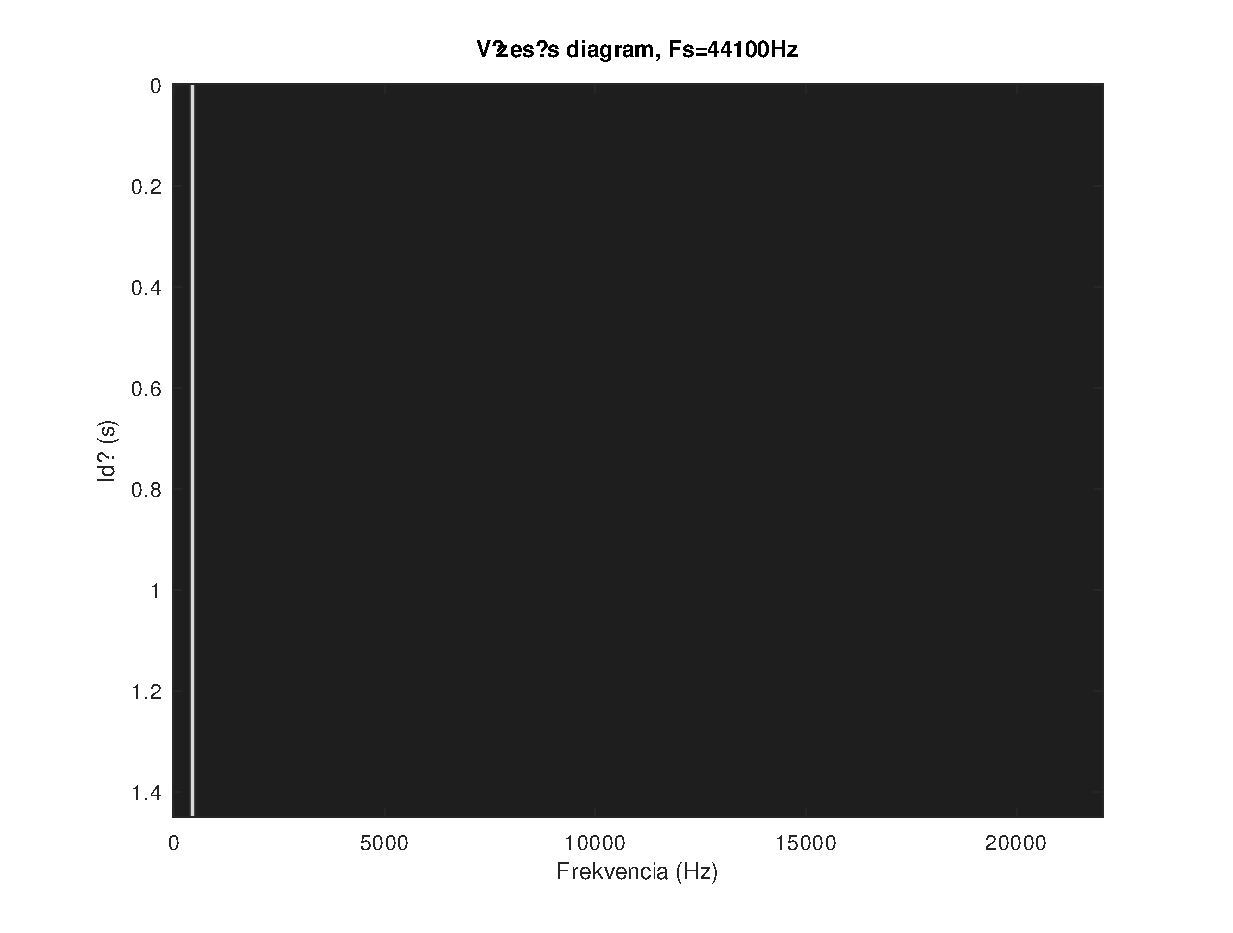
\includegraphics[width=8cm]{figures/modulaciok_workshop_waterfall.eps}
\caption{440 Hz-es szinusz függvény ábrázolása frekvenciatartományban}
\label{fig:waterfall}
\end{center}
\end{figure}

A vízesés diagram 0-tól a mintavételi frekvencia feléig ábrázolja a frekvenciakomponenseket, az ábrán láthatjuk a konstans szinusz jel képét 440 Hz-nél. Próbálkozzunk meg a jel manipulálásával, hallgassuk meg, ábrázoljuk frekvenciatartományban!\\
\lstinline{y = ( 1 - ( 1 / l ) * t ) .* sin( t * f * 2 * pi ); % Fokozatosan halkulo jel } \\
\lstinline{y = sin( t .* ( f * t ) * 2 * pi ); % Valtozo frekvenciaju szinusz } \\
\lstinline{y = sin( t * f * 2 * pi ) + sin( t * 1.5*f * 2 * pi ) ; % Tobb szinusz osszege }
\\
Megpróbálhatunk fehér zajt generálni, vagy hangfilet betölteni is. \\
\lstinline{y = rand( N, 1 ) ; % N elemu zaj}  \\
\lstinline{[y,Fs] = audioread( 'akkord.wav' ); N = length( y ); l=N/Fs; % WAV file beolvasasa}


\clearpage

\subsection{Keverés}


\begin{figure}[H]
\label{fig:keverok}
\centering
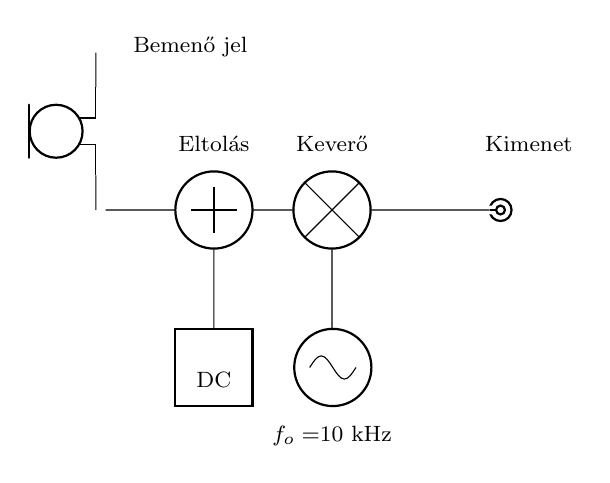
\begin{tikzpicture}

	\draw
	(5,0)node[bnc, xscale=-1] (bnc){}	
	(0,0) to[mic, name=M] ++(0,2)
	(1.2,1.7) node[label={[font=\footnotesize]above:Bemenő jel}] {}

	(3,-2.5) node[label={[font=\footnotesize]below:$f_o=$10 kHz}] {}
	
	(3,0.5) node[label={[font=\footnotesize]above:Keverő}] {}
	(1.5,0.5) node[label={[font=\footnotesize]above:Eltolás}] {}
	(5.5,0.5) node[label={[font=\footnotesize]above:Kimenet}] {}
	(1.5,-2.5) node[label={[font=\footnotesize]above:DC}] {}
	(0,0)[mic]node(mic){}
	(3,0)[mixer] node(mix){}	
	
	(1.5,0)[adder] node(add){}	
	(3.5,-2)[oscillator] node(osc){}	
	(1.5,-2)[twoportshape] node(dc){}
	
	
	(mic) to [short] ++(1,0) 
	
	(2,0) to [short] ++(0.5,0) 
	(3,-1.5) to [short] (3,-0.5)
	(1.5,-1.5) to [short] (1.5,-0.5)
	(3.5,0) to [short] (5,0)
	
	;
    \end{tikzpicture}
\caption{
A keverő blokkvázlata} 
\end{figure}

Amikor egy jelet egy szinusz oszcillátor jelével keverünk (szorzunk), a jel megjelenik a frekvenciatartományban a két frekvencia összegeként és különbségeként. Ha pl a két jel egy $\omega_1$ frekvenciájú koszinusz vivő, és egy $\omega_2$ frekvenciájú koszinusz moduláló jel, a modulációs tétel alapján:

\begin{equation}
\cos(\omega_1t) \cdot \cos(\omega_2t) = \frac{1}{2}\cos(\omega_1t+\omega_2t) +  \frac{1}{2}\cos(\omega_1t - \omega_2t)
\end{equation}

Nézzük meg a gyakorlatban, próbáljuk meg az \textit{akkord.wav} hangfilet keverni, például egy 10 kHz-es szinusz jellel!


\begin{lstlisting}[frame=single,language=matlab,caption=Keverés]
[a,Fs] = audioread('akkord.wav'); N=length(a);
f = 10000; % 10 kHz-es lesz a vivo jel
t = ( 1:N )' ./ Fs;
b = sin( t * f * 2 * pi );

m = 0.75; % modulacios index
dc_offset = (1 + 1-m) * max(a);
a_dc = a + dc_offset; % dc eltolas

y = a_dc .* b; % keveres (a .* b)

wf(y, Fs);
\end{lstlisting}

Fontos, hogy eltoljuk az eredeti jelet úgy, hogy a moduláló jel ne menjen 0 szint alá, különben túlmoduláljuk a vivő jelet. A vivő és moduláló jel amplitúdójának kapcsolatát a modulációs mélységgel jellemezzük. 

Vajon hogyan kapjuk vissza a kevert jelből az eredeti információt?

\clearpage

\subsection{IQ moduláció}



\begin{figure}[H]
\label{fig:iq}
\centering
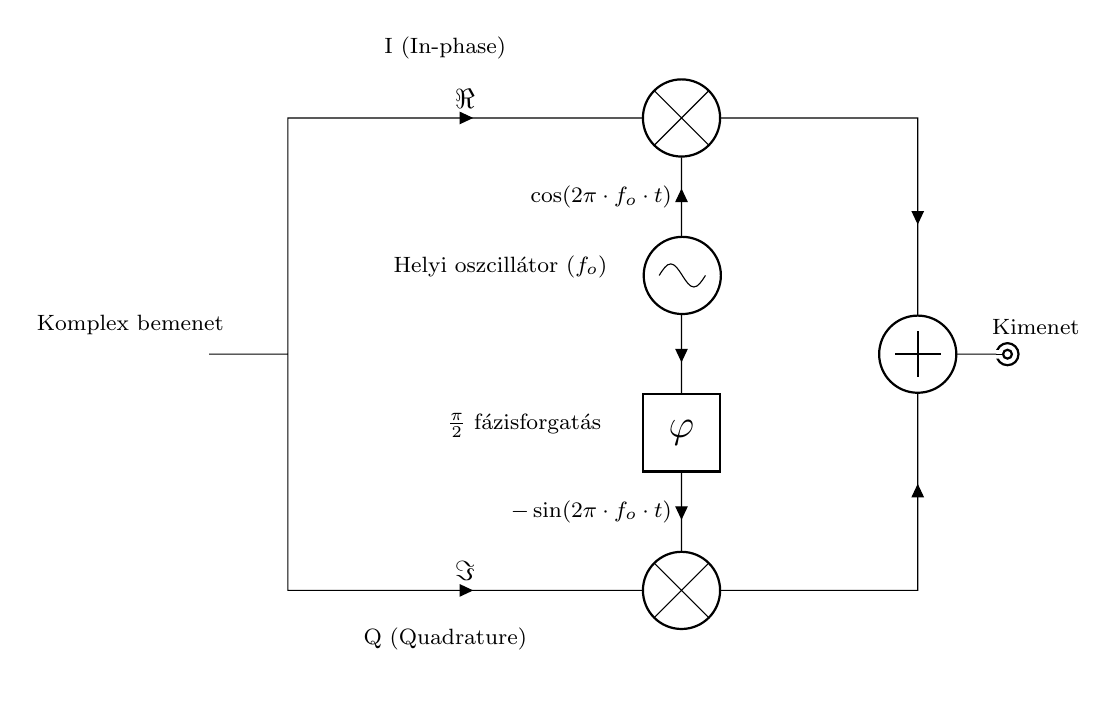
\begin{tikzpicture}

	\draw
	(10,-3)node[bnc, xscale=-1] (bnc){}	
	(-1,-3) node[label={[font=\footnotesize]above:Komplex bemenet}] {}
	
	(3.7,-1.5) node[label={[font=\footnotesize]below:Helyi oszcillátor ($f_o$)}] {}
	(4,-3.5) node[label={[font=\footnotesize]below:$\frac{\pi}{2}$ fázisforgatás}] {}
	(3,0.5) node[label={[font=\footnotesize]above:I (In-phase)}] {}
	(3,-7) node[label={[font=\footnotesize]above:Q (Quadrature)}] {}
	(10.5,-3) node[label={[font=\footnotesize]above:Kimenet}] {}
	
	(0, -3) to [short] ++(1,0) 
	(1,-3) to [short] ++(0,3) to [short, i=$\Re$] ++(4.5,0) 
	(1,-3) to [short] ++(0,-3) to [short, i=$\Im$] ++(4.5,0) 	
	
	(6,-1.5) to [short, i=\footnotesize $\cos(2\pi \cdot f_o \cdot t)$] (6,-0.5)
	
	(6,-2.5) to [short, i=\phantom{}] (6,-3.5)
	
	(6,-4.5) to [short, i>_=\footnotesize $-\sin(2\pi \cdot f_o \cdot t)$] (6,-5.5)
	
	(6.5,0) to [short] ++(2.5,0) to [short, i=\phantom{}] ++(0,-2.5) 
	(6.5,-6) to [short] ++(2.5,0) to [short, i=\phantom{}] ++(0,2.5) 
	(9.5,-3) to [short] ++(0.5,0)
	(6,0)[mixer] node(mixa){}	
	(6,-6)[mixer] node(mixb){}	
	

	(6.5,-2)[oscillator] node(osc){}	
	(6,-4)[phaseshiftershape] node(phas){}	
	
	(9,-3)[adder] node(add){}	
	
	;
    \end{tikzpicture}
\caption{
Az IQ modulátor blokkvázlata} 
\end{figure}

Az IQ modulátornál egy komplex jellel moduláljuk a vivő frekvenciát. Ezzel a módszerrel az alapsávi jelet egy komplex fazorként ábrázolhatjuk, és ez nagyban megkönnyíti a modulációs műveletek elvégzését.

\subsubsection{Fázismoduláció}

Vegyük át újra hogy is néz ki egy szinusz.
\begin{equation}
y(t) = A \cdot \sin{ ( f\cdot t +  \phi   ) }
\end{equation}
A képletben lévő amplitúdót amplitúdómodulációban, a frekvenciát frekvenciamodulációban használjuk, a fázist pedig fázismodulációban. Talán a fázismodulációt a legnehezebb megfogni élettapasztalatból, mivel a fülünkkel nem halljuk ki a jelek fázisát -- furcsa is lenne ha egy méterrel távolabbról másnak hallanánk mások hangját. A fázis jelen esetben is nehezen értelmezhető, mivel a kiadott jel úgymond elveszik, nincs mihez hasonlítani első közelítésben majd vevő oldalon a fázist. A probléma feloldása az, hogy egyrészt eltárolhatjuk a jel mintáit majd vevőoldalon, illetve a fázist tudja majd a vevő a saját, azonos frekvencián futó oszcillátorához képest mérni. Különböző frekvenciákhoz nincs értelme fázist mérni általában, mert a különböző frekvencia miatt fázisban úgyis elmásznak egymástól.
\clearpage
Készítsünk fázismodulátort IQ moduláció segítségével! Legyen az átvinni kívánt (moduláló) jel $x(t)$ (ügyelve arra, hogy $\vert x(t) \vert<1$)! Ekkor a $c(t)$ komplex vektor hossza $\vert c(t) \vert = 1$, fázisa pedig a modulált jel pillanatnyi értéke ($\arg\left(c(t)\right)=x(t) \cdot \pi$). Így a jel 1 értéke a $\pi$ fázishoz kerül. A $c(t)$ jelet az Euler alakkal könnyen előállíthatjuk: $c(t)=e^{j \cdot \pi \cdot x(t)}$.

\begin{figure}[H]
\begin{center}
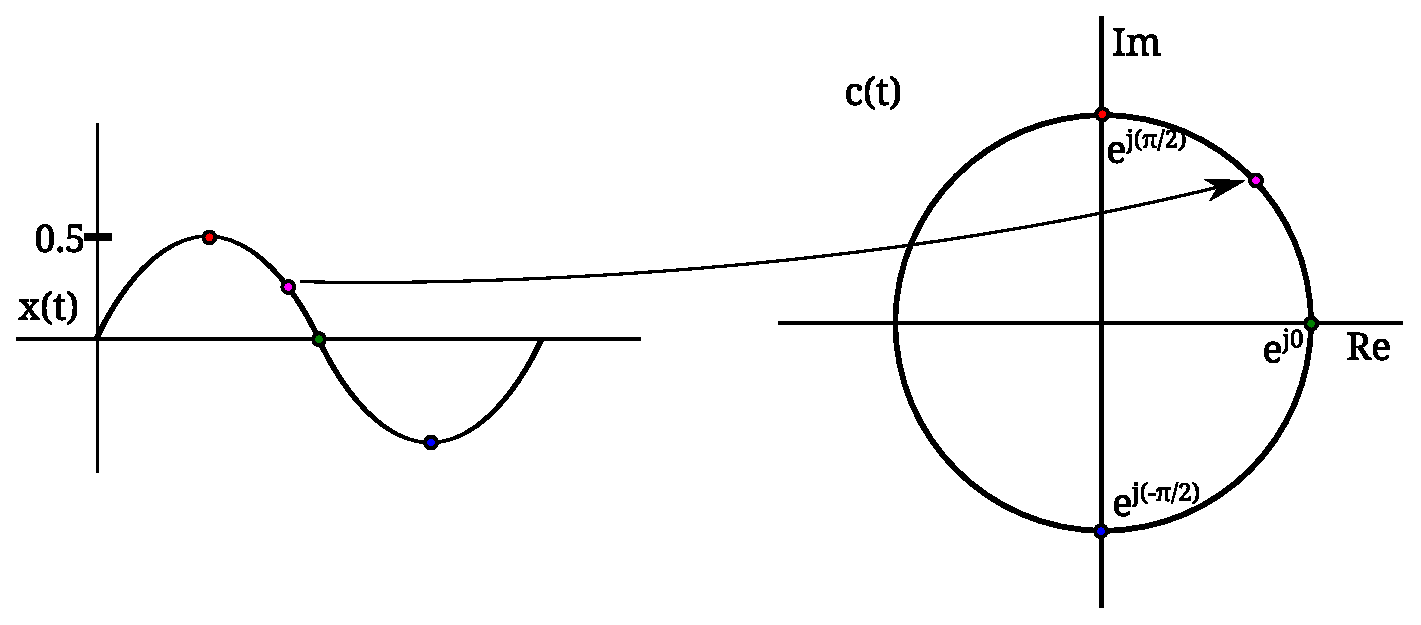
\includegraphics[width=13cm]{figures/modulaciok_workshop_pm.eps}
\caption{Fázisok előállítása a moduláló jelből}
\label{fig:pm}
\end{center}
\end{figure}

Az IQ keveréshez ennek a komplex jelnek a valós részét az in-phase $\cos(2\pi \cdot f_o \cdot t)$, a képzetes részét a quadrature $-\sin(2\pi \cdot f_o \cdot t)$ oszcillátor jellel moduláljuk (szorozzuk), majd összeadjuk. Kész is a modulált jel!

\begin{figure}[H]
\begin{center}
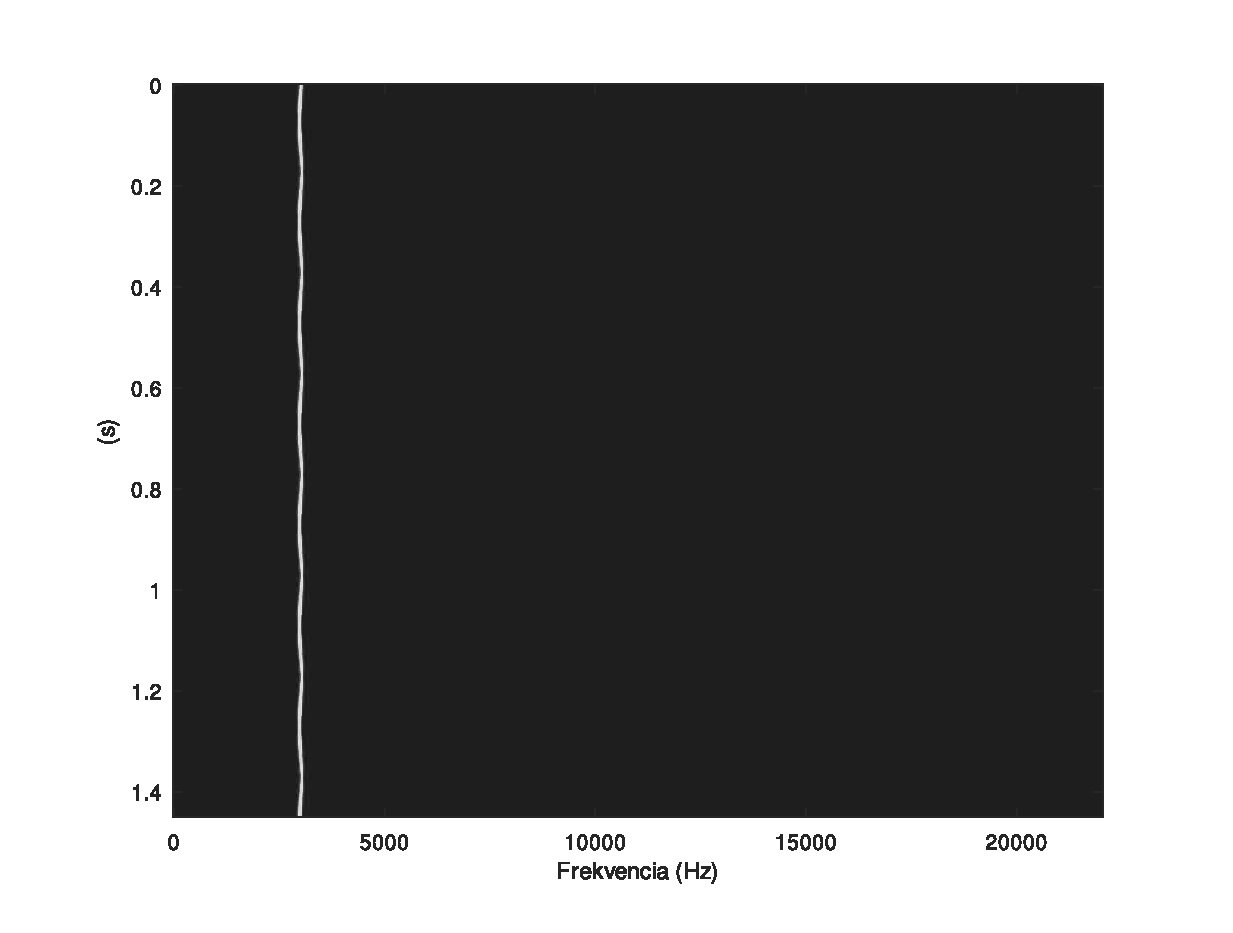
\includegraphics[width=8cm]{figures/modulaciok_workshop_phase.eps}
\caption{Az előállított fázismodulált jel}
\label{fig:phase}
\end{center}
\end{figure}
\clearpage
\begin{lstlisting}[frame=single,language=matlab,caption=Fázismoduláció IQ modulátorral]
Fs = 44100; % mintaveteli freki
l = 1.5; % minta hossza masodpercben
N = l * Fs; % mintak szama
t = ( 1:N )' ./ Fs; % Ido oszlopvektora

f = 5; % eredeti jel frek
x =  sin( t * f * 2 * pi ) .* 0.5; % ez lesz az atvinni kivant jel (1/2 amplitudo)

c = ones(N,1); % N meretu vektor letrehozasa es feltoltese 1-essel
for i=1:N
  c(i) = exp( j * pi * x(i) ); % fazismodulalt jel letrehozasa
  % e^(2pi*j*x/2), mert nem szeretnenk a korbeforgassal atlapolodni
end

fo = 3000; % oszcillator frek
oi =  cos( t * fo * 2 * pi ); % in-phase oszcillator
oq = -sin( t * fo * 2 * pi ); % quadrature oszcillator

y = oq .* imag(c) + oi .* real(c); % IQ keveres

figure(1);
plot(t, y);
figure(2);
wf(y, Fs);
\end{lstlisting}

Ez alapján készítsünk el egy FM modulátort! Nagyon hasonlít az előzőhöz, csak itt a komplex vektor forgásának frekvenciája változik.

\subsection{Újramintavételezés}

Próbáljuk ki hangfileokkal! Ügyeljünk arra, hogy a FM sávszélessége nagy lesz, ezért nagyobb helyre lesz szükségünk a frekvenciatartományban. Ha megváltoztatjuk a mintavételi frekvenciát és a hangot újramintavételezzük ez alapján, ki tudjuk terjeszteni a frekvenciatartomány méretét. \\
Vigyázzunk, hogy $n$-szeres mintavételi frekvenciánál a minták száma is $n$-szeresére változik, és ez nagyon megnövelheti a számítási időt. \\
Az újramintavételezés a \textit{resample(x, p, q)} függvénnyel tehető meg, ami $\frac{p}{q}$-szorosára változtatja a mintavételi frekvenciát (ehhez be kell tölteni a signal csomagot). Ne felejtsük a $F_s$ változót is beállítani!
\begin{lstlisting}[frame=single,language=matlab,caption=Újramintavételezés]
[x,Fs] = audioread('voice.wav');
% Ujramintavetelezes -> nagyobb frekitartomany
Fs = Fs * 4;
x = resample(x, 4, 1);
N = length( x ); l = N / Fs;
\end{lstlisting}

\end{document}



